\chapter{Linear systems}

\section{Introduction}

\begin{definition}[Non-Singular Matrix]\index{Non-Singular Matrix}
    A coefficient matrix \( A \) is \term{non-singular} if and only if \[
        \exists A^{-1} \text{ such that } A A^{-1} = A^{-1} A = I
    \]
\end{definition}

\begin{remark}
    Some facts
    \begin{itemize}
        \item \( A\vec{x} = \vec{b} \) has a \textbf{unique} solution if and only if \( A \) is non-singular.
        \item \( A \) is non-singular if and only if \( \det(A) \neq 0 \).
    \end{itemize}
\end{remark}

In the contrast, a singular matrix is one that is not invertible.

\begin{proposition}
    If \( \exists z \neq 0 \) such that \( A z = 0 \), then \( A \) is singular.
\end{proposition}

\begin{remark}
    Suppose exists \( y \) such that \( A \vec{y} = \vec{b} \), then \( y + \alpha z \) solves \( A \vec{x} = \vec{b} \) may not be a solution.

    For example, \[
        \begin{pmatrix} 1 & 2 \\ 3 & 4 \end{pmatrix} \begin{pmatrix} x_1 \\ x_2 \end{pmatrix} = \begin{pmatrix} 3 \\ 7 \end{pmatrix}
    \] has no solution.
\end{remark}

We will stick to the case where \( A \) is non-singular.

\subsection{Cramer's Rule}

\begin{definition}[Cramer's Rule]\index{Cramer's Rule}
    For a linear system \( A \vec{x} = \vec{b} \), the solution is \[
        x_i = \frac{\det(A_i)}{\det(A)}
    \] where \( A_i \) is the matrix obtained by replacing the \( i \)th column of \( A \) with \( b \).
\end{definition}

\begin{remark}
    Cramer's Rule is not practical for large systems, as it requires \( n+1 \) determinants.
\end{remark}

\section{Gaussian Elimination}

Alternatively, we can compute \( A^{-1} \) and then \( x = A^{-1} b \).

To solve for \( A^{-1} \), we solve for \( AY = I \), then \( x = Yb \).

For \( i = 1 \) to \( n \):
use some method to solve \( Ay_i = e_i = \begin{pmatrix} 0 \\ \vdots \\ 1 \\ \vdots \\ 0 \end{pmatrix} \).

\subsection{Intuition}

\subsubsection{Case I}

Suppose \( A \) is non-singular diagonal matrix, \[
    A = \begin{pmatrix}
        a_1    & 0      & \cdots & 0      \\
        0      & a_2    & \cdots & 0      \\
        \vdots & \vdots & \ddots & \vdots \\
        0      & 0      & \cdots & a_n
    \end{pmatrix}
\]

We must have \( \begin{cases}
    a_{ij} \neq 0 & \text{if } i = j    \\
    a_{ij} = 0    & \text{if } i \neq j
\end{cases} \)

Indeed, since \( A \) non-singular, \( \det(A) \neq 0 \), and since \( A \) diagonal, \( \det(A) = a_1 a_2 \cdots a_n \neq 0 \). None of the diagonal elements can be zero.

Then, for \( Ax = b \), we have \( x_i = b_i / a_{i,i} \). We can solve this within a single loop.

\begin{algorithmic}
    \For{\( i = 1 \) to \( n \)}
    \State \( x_i = b_i / a_{i,i} \)
    \EndFor
\end{algorithmic}

To count the number of operations, we define a new unit of operation, the \term{flop}.

\begin{definition}[FLOP]\index{FLOP}
    A \term{FLOP} is a \textbf{F}loating-point \textbf{L}inear \textbf{O}peration. This is a single arithmetic operation on floating-point numbers.
\end{definition}

\begin{example}
    For the above algorithm, each iteration require 1 FLOP -- a division. Thus, we require \( n \) FLOPs to solve the system.
\end{example}

\subsubsection{Case II}

Suppose \( A \) is non-singular lower-triangular, \[
    A = \begin{pmatrix}
        a_{11} & 0      & \cdots & 0      \\
        a_{21} & a_{22} & \cdots & 0      \\
        \vdots & \vdots & \ddots & \vdots \\
        a_{n1} & a_{n2} & \cdots & a_{nn}
    \end{pmatrix}
\]
We must have \( \begin{cases}
    a_{ij} = 0    & \text{if } i < j                     \\
    a_{ii} \neq 0 & \text{since } A \text{ non-singular}
\end{cases} \)

\begin{itemize}
    \item \( x_1 = b_1 / a_{1,1} \)
    \item \( x_2 = (b_2 - a_{2,1} x_1) / a_{2,2} \)
    \item \( x_3 = (b_3 - a_{3,1} x_1 - a_{3,2} x_2) / a_{3,3} \)
    \item \( \vdots \)
    \item \( \displaystyle x_i = \left( b_i - \sum_{j=1}^{i-1} a_{ij} x_j \right) / a_{ii} \)
\end{itemize}

This algorithm is called \term{forward substitution}.

\begin{algorithm}[H]
    \begin{algorithmic}
        \Function{ForwardSubstitution}{$A, b$}
        \For{\( i = 1 \) \To \( n \)}
        \State \( sum = 0 \)
        \For{\( j = 1 \) \To \( i-1 \)}
        \State \( sum = sum + a_{ij} \cdot x_j \)
        \EndFor
        \State \( x_i = (b_i - sum) / a_{ii} \)
        \EndFor
        \State \Return \( x \)
        \EndFunction
    \end{algorithmic}
\end{algorithm}

We have the operation count \[
    \sum_{i=1}^n \left[ \left( \sum_{j=1}^{i-1} 2 \right) + 2 \right] = n^2 + \Theta(n) \text{ FLOPs}.
\]

\subsubsection{Case III}

Suppose \( A \) is non-singular upper-triangular, \[
    A = \begin{pmatrix}
        a_{11} & a_{12} & \cdots & a_{1n} \\
        0      & a_{22} & \cdots & a_{2n} \\
        \vdots & \vdots & \ddots & \vdots \\
        0      & 0      & \cdots & a_{nn}
    \end{pmatrix}
\]

We must have \( \begin{cases}
    a_{ij} = 0    & \text{if } i > j                     \\
    a_{ii} \neq 0 & \text{since } A \text{ non-singular}
\end{cases} \)

\begin{itemize}
    \item \( x_n = b_n / a_{n,n} \)
    \item \( x_{n-1} = (b_{n-1} - a_{n-1,n} x_n) / a_{n-1,n-1} \)
    \item \( x_{n-2} = (b_{n-2} - a_{n-2,n} x_n - a_{n-2,n-1} x_{n-1}) / a_{n-2,n-2} \)
    \item \( \vdots \)
    \item \( \displaystyle x_i = \left( b_i - \sum_{j=i+1}^{n} a_{ij} x_j \right) / a_{ii} \)
\end{itemize}

This algorithm is called \term{backward substitution}.

\begin{algorithm}[H]
    \begin{algorithmic}
        \Function{BackwardSubstitution}{$A, b$}
        \For{\( i = n \) \DownTo \( 1 \)}
        \State \( sum = 0 \)
        \For{\( j = i+1 \) \To \( n \)}
        \State \( sum = sum + a_{ij} \cdot x_j \)
        \EndFor
        \State \( x_i = (b_i - sum) / a_{ii} \)
        \EndFor
        \State \Return \( x \)
        \EndFunction
    \end{algorithmic}
\end{algorithm}

The operation count will be the same as for forward substitution, \[
    n^2 + \Theta(n) \text{ FLOPs}.
\]

\subsubsection{Case IV}

What if \( A \) is dense? We can use Gaussian elimination to reduce \( A \) to a triangular form.

\subsection{Gaussian Elimination}

\begin{example}
    Suppose we want to solve the linear system \[
        \begin{pmatrix}
            2 & 1 & 1 & 0 \\
            4 & 3 & 3 & 1 \\
            8 & 7 & 9 & 5 \\
            6 & 7 & 9 & 8
        \end{pmatrix}
        \begin{pmatrix}
            x_1 \\ x_2 \\ x_3 \\ x_4
        \end{pmatrix}
        =
        \begin{pmatrix}
            1 \\ 1 \\ -1 \\ 3
        \end{pmatrix}
    \]

    Recall from linear algebra that elementary operations do not change the solution to the system. We can use the elementary row operation \[
        R_j = R_j - m \cdot R_i
    \] to convert \( A \) to an upper-triangular form.

    \begin{enumerate}
        \item \( R_2 = R_2 - 2 \cdot R_1 \qquad R_3 = R_3 - 4 \cdot R_1 \qquad R_4 = R_4 - 3 \cdot R_1 \)
              \[
                  \begin{pmatrix}
                      2 & 1 & 1 & 0 \\
                      0 & 1 & 1 & 1 \\
                      0 & 3 & 5 & 5 \\
                      0 & 4 & 6 & 8 \\
                  \end{pmatrix}
                  \vec{x}
                  =
                  \begin{pmatrix}
                      1 \\ -1 \\ -5 \\ -6
                  \end{pmatrix}
              \]

        \item \( R_3 = R_3 - 3 \cdot R_2 \qquad R_4 = R_4 - 4 \cdot R_2 \)

              \[
                  \begin{pmatrix}
                      2 & 1 & 1 & 0 \\
                      0 & 1 & 1 & 1 \\
                      0 & 0 & 2 & 2 \\
                      0 & 0 & 2 & 4 \\
                  \end{pmatrix}
                  \vec{x}
                  =
                  \begin{pmatrix}
                      1 \\ -1 \\ -2 \\ -2
                  \end{pmatrix}
              \]

        \item \( R_4 = R_4 - R_3 \)

              \[
                  \begin{pmatrix}
                      2 & 1 & 1 & 0 \\
                      0 & 1 & 1 & 1 \\
                      0 & 0 & 2 & 2 \\
                      0 & 0 & 0 & 2 \\
                  \end{pmatrix}
                  \vec{x}
                  =
                  \begin{pmatrix}
                      1 \\ -1 \\ -2 \\ 0
                  \end{pmatrix}
              \]
    \end{enumerate}

    We now have a triangular system. We can use backward substitution to solve for \( x \). \[
        \vec{x} = \begin{pmatrix}
            1 \\ 0 \\ -1 \\ 0
        \end{pmatrix}
    \]

    How could we program this algorithm?
\end{example}

\begin{algorithm}[H]
    \begin{algorithmic}[1]
        \Function{GaussianElimination}{$A, b$}
        \State \( n \gets \text{size}(A) \)
        \State \( ms \gets \texttt{[]} \) \Comment{Multipliers}
        \For{\( i \gets 1 \) \To \( n-1 \)} \Comment{Going down the diagonal}
        \For{\( j \gets i+1 \) \To \( n \)} \Comment{Below the diagonal}
        \State \( m \gets A_{j,i} / A_{i,i} \)
        \State \( ms[j,i] \gets m \)
        % \State \( A_{j,i} = 0 \)
        \For{\( k \gets i+1 \) \To \( n \)}
        \State \( A_{j,k} \gets A_{j,k} - m \cdot A_{i,k} \)
        \EndFor
        % \State \( b_j = b_j - m \cdot b_i \)
        \EndFor
        \EndFor
        \State \Return \( A, ms \)
        \EndFunction
    \end{algorithmic}
\end{algorithm}

\begin{remark}
    The reason not to update \( b \), but rather to store the multipliers, is that often in practice we have multiple right-hand sides. We can then use the same multipliers to solve for all right-hand sides.
\end{remark}

What is the operation count for Gaussian elimination? We consider only the operations on \( A \), since the operations on \( b \) are negligible.

\begin{itemize}
    \item The inner most operation occurs on line 9, with 2 FLOPs.
    \item They are repeated for \( k = i+1 \) to \( n \), \( \sum_{k=i+1}^n 2 \) FLOPs.
    \item There is one more operation on line 6, with 1 FLOP.
    \item The \( j \) loop is repeated for \( j = i+1 \) to \( n \), \( \sum_{j=i+1}^n \left( 1 + \sum_{k=i+1}^n 2 \right) \) FLOPs.
    \item The outer loop is repeated for \( i = 1 \) to \( n-1 \), \( \sum_{i=1}^{n-1} \left( 1 + \sum_{j=i+1}^n \left( 1 + \sum_{k=i+1}^n 2 \right) \right) \) FLOPs.
\end{itemize}

We then simplify
\begin{align*}
    \operatorname{FLOP}
     &
    = \sum_{i=1}^{n-1} \left( 1 + \sum_{j=i+1}^n \left( 1 + \sum_{k=i+1}^n 2 \right) \right)
    \\
     &
    = \sum_{i=1}^{n-1} \left( 1 + \sum_{j=i+1}^n \left( 1 + 2(n - i) \right) \right)
    \\
     &
    = \sum_{i=1}^{n-1} \left[ (n - i) (1 + 2(n - i)) \right]
\end{align*}

Taking \( m = n - i \), we have
\begin{align*}
    \operatorname{FLOP}
     &
    = \sum_{m=1}^{n-1} m (1 + 2m)
    \\
     &
    = \left( \sum_{m=1}^{n-1} m \right) + 2 \left( \sum_{m=1}^{n-1} m^2 \right)
    \\
     &
    = \frac{n(n-1)}{2} + 2 \cdot \frac{2n^3 - 3n^2 + n}{6}
    \\
     &
    = \frac{2n^3}{3} - \frac{n^2}{2} - \frac{n}{6}
    \\
     & = \frac{2}{3} n^3 + \Theta(n^2) \text{ FLOPs}
\end{align*}

\subsection{Gauss Transforms}

\begin{definition}[Gauss Transformation Matrix]
    A \term{\( n \times n \) Gauss transformation matrix} \( m_R \) is defined as \[
        m_R = I - \vec{m}_r \cdot \vec{e}_r^\top
    \] where \( m_R \in \R^n \) and \[
        \vec{m}_r = \begin{pmatrix}
            0 \\ \vdots \\ 0 \\ m_{r+1,r} \\ m_{r+2,r} \\ \vdots \\ m_{n,r}
        \end{pmatrix}
        \qquad \text{and} \qquad
        \vec{e}_r = \begin{pmatrix}[l]
            0 \\ \vdots \\ 0 \\ 1 \text{ \(r\)th row} \\ 0 \\ \vdots \\ 0
        \end{pmatrix}
    \]
\end{definition}

\begin{remark}
    \begin{align*}
        M_r
         &
        = I - m_r e_r^\top
        \\
         &
        = I - \begin{pmatrix}
                  0 &        &           &   &   &        &   \\
                    & \ddots &           &   &   &        &   \\
                    &        & 0         &   &   &        &   \\
                    &        & m_{r+1,r} & 0 &   &        &   \\
                    &        & m_{r+2,r} & 0 & 0 &        &   \\
                    &        & \vdots    &   &   & \ddots &   \\
                    &        & m_{n,r}   &   &   &        & 0
              \end{pmatrix}
        % \\
        %  &
        = \begin{pmatrix}
              1 &        &            &   &   &        &   \\
                & \ddots &            &   &   &        &   \\
                &        & 1          &   &   &        &   \\
                &        & -m_{r+1,r} & 1 &   &        &   \\
                &        & -m_{r+2,r} & 0 & 1 &        &   \\
                &        & \vdots     &   &   & \ddots &   \\
                &        & -m_{n,r}   &   &   &        & 1
          \end{pmatrix}
    \end{align*}
\end{remark}

\begin{note}[Properties of Gauss Transforms]
    Gauss transforms have nice properties:
    \begin{enumerate}
        \item For indices \( r \leq s \), \[
                  M_r M_s = I - \vec{m}_r \vec{e}_r^\top - \vec{m}_s \vec{e}_s^\top
              \] (not a Gauss transform)

        \item \[
                  M_r^{-1} = I + \vec{m}_r \vec{e}_r^\top
              \] (is a Gauss transform)

        \item For any \(n-\)vector \( \vec{v} = [v_1, v_2, \ldots, v_n]^\top \), \begin{align*}
                  M_r \vec{v}
                   &
                  = ( I - \vec{m}_r \vec{e}_r^\top) \vec{v}
                  \\
                   &
                  = \vec{v} - \vec{m}_r (\vec{e}_r^\top \vec{v})
                  \\
                   &
                  = \vec{v} - v_r \vec{m}_r
                  \\
                   &
                  = \begin{pmatrix}
                        v_1 \\ \vdots \\ v_{r} \\ v_{r+1} - v_r m_{r+1,r} \\ \vdots \\ v_n - v_r m_{n,r}
                    \end{pmatrix}
              \end{align*}
    \end{enumerate}
\end{note}

\begin{example}
    Suppose \[
        A = \begin{pmatrix}
            2 & 1 & 1 & 0 \\ 4 & 3 & 3 & 1 \\ 8 & 7 & 9 & 5 \\ 6 & 7 & 9 & 8
        \end{pmatrix}
    \]

    \begin{itemize}
        \item Choose \[
                  m_1 = \begin{pmatrix}
                      0 \\ 2 \\ 4 \\ 3
                  \end{pmatrix}
                  \implies
                  M_1 = \begin{pmatrix}
                      1 & 0 & 0 & 0 \\ -2 & 1 & 0 & 0 \\ -4 & 0 & 1 & 0 \\ -3 & 0 & 0 & 1
                  \end{pmatrix}
              \]

              We have \[
                  M_1 A
                  =
                  \begin{pmatrix}
                      1 & 0 & 0 & 0 \\ -2 & 1 & 0 & 0 \\ -4 & 0 & 1 & 0 \\ -3 & 0 & 0 & 1
                  \end{pmatrix}
                  \begin{pmatrix}
                      2 & 1 & 1 & 0 \\ 4 & 3 & 3 & 1 \\ 8 & 7 & 9 & 5 \\ 6 & 7 & 9 & 8
                  \end{pmatrix}
                  =
                  \begin{pmatrix}
                      2 & 1 & 1 & 0 \\ 0 & 1 & 1 & 1 \\ 0 & 3 & 5 & 5 \\ 0 & 4 & 6 & 8
                  \end{pmatrix}
              \]

        \item Choose \[
                  m_2 = \begin{pmatrix}
                      0 \\ 0 \\ 3 \\ 4
                  \end{pmatrix}
                  \implies
                  M_2 = \begin{pmatrix}
                      1 & 0 & 0 & 0 \\ 0 & 1 & 0 & 0 \\ 0 & -3 & 1 & 0 \\ 0 & -4 & 0 & 1
                  \end{pmatrix}
              \]

              We have \[
                  M_2 M_1 A
                  =
                  \begin{pmatrix}
                      1 & 0 & 0 & 0 \\ 0 & 1 & 0 & 0 \\ 0 & -3 & 1 & 0 \\ 0 & -4 & 0 & 1
                  \end{pmatrix}
                  \begin{pmatrix}
                      2 & 1 & 1 & 0 \\ 0 & 1 & 1 & 1 \\ 0 & 3 & 5 & 5 \\ 0 & 4 & 6 & 8
                  \end{pmatrix}
                  =
                  \begin{pmatrix}
                      2 & 1 & 1 & 0 \\ 0 & 1 & 1 & 1 \\ 0 & 0 & 2 & 2 \\ 0 & 0 & 2 & 4
                  \end{pmatrix}
              \]

        \item Choose \[
                  m_3 = \begin{pmatrix}
                      0 \\ 0 \\ 0 \\ 1
                  \end{pmatrix}
                  \implies
                  M_3 = \begin{pmatrix}
                      1 & 0 & 0 & 0 \\ 0 & 1 & 0 & 0 \\ 0 & 0 & 1 & 0 \\ 0 & 0 & -1 & 1
                  \end{pmatrix}
              \]

              We have \[
                  M_3 M_2 M_1 A
                  =
                  \begin{pmatrix}
                      1 & 0 & 0 & 0 \\ 0 & 1 & 0 & 0 \\ 0 & 0 & 1 & 0 \\ 0 & 0 & -1 & 1
                  \end{pmatrix}
                  \begin{pmatrix}
                      2 & 1 & 1 & 0 \\ 0 & 1 & 1 & 1 \\ 0 & 0 & 2 & 2 \\ 0 & 0 & 2 & 4
                  \end{pmatrix}
                  =
                  \begin{pmatrix}
                      2 & 1 & 1 & 0 \\ 0 & 1 & 1 & 1 \\ 0 & 0 & 2 & 2 \\ 0 & 0 & 0 & 2
                  \end{pmatrix}
              \]
    \end{itemize}

    We end up with an upper-triangular matrix \[
        U = M_3 M_3 M_1 A = \begin{pmatrix}
            2 & 1 & 1 & 0 \\ 0 & 1 & 1 & 1 \\ 0 & 0 & 2 & 2 \\ 0 & 0 & 0 & 2
        \end{pmatrix}
    \]

    This also implies \begin{align*}
        A = (M_3 M_2 M_1)^{-1} U
         &
        = M_1^{-1} M_2^{-1} M_3^{-1} U
        \\
         &
        = (I + \vec{m}_1 \vec{e}_1^\top) (I + \vec{m}_2 \vec{e}_2^\top) (I + \vec{m}_3 \vec{e}_3^\top) U
         & \text{by property 2}
        \\
         &
        =
        \begin{pmatrix}
            1 & 0 & 0 & 0 \\ 2 & 1 & 0 & 0 \\ 4 & 3 & 1 & 0 \\ 3 & 4 & 1 & 1
        \end{pmatrix} U
    \end{align*}
    and we have an anti lower-triangular matrix \[
        L = \begin{pmatrix}
            1 & 0 & 0 & 0 \\ 2 & 1 & 0 & 0 \\ 4 & 0 & 1 & 0 \\ 3 & 0 & 0 & 1
        \end{pmatrix}
    \]

    We can think of Gaussian Elimination as factoring \( A \) into \( LU \), where \( L \) is lower-triangular and \( U \) is upper-triangular.

    Verify: \[
        LU =
        \begin{pmatrix}
            1 & 0 & 0 & 0 \\ 2 & 1 & 0 & 0 \\ 4 & 3 & 1 & 0 \\ 3 & 4 & 1 & 1
        \end{pmatrix}
        \begin{pmatrix}
            2 & 1 & 1 & 0 \\ 0 & 1 & 1 & 1 \\ 0 & 0 & 2 & 2 \\ 0 & 0 & 0 & 2
        \end{pmatrix}
        =
        \begin{pmatrix}
            2 & 1 & 1 & 0 \\ 4 & 3 & 3 & 1 \\ 8 & 7 & 9 & 5 \\ 6 & 7 & 9 & 8
        \end{pmatrix}
    \]
\end{example}

\section{Solving System of Linear Equations}

\subsection{LU Factorization}

How to solve \( A \vec{x} = \vec{b} \)?

\begin{enumerate}
    \item Factor \( A = LU \)

          The operation cont is \[
              \frac{2}{3} n^3 + \Theta(n^2) \text{ FLOPs}
          \]

          Then, we have \[
              L(U \vec{x}) = \vec{b}
          \]

          Let \( \vec{y} = U\vec{x} \), we have an triangular system \[
              L \vec{y} = \vec{b}
          \]

    \item Solve \( L \vec{y} = \vec{b} \) for \( \vec{y} \) using forward substitution.

          The operation count is \[
              n^2 + \Theta(n) \text{ FLOPs}
          \]

          Then, we have \[
              U \vec{x} = \vec{y}
          \]

    \item Solve \( U \vec{x} = \vec{y} \) for \( \vec{x} \) using backward substitution.

          The operation count is \[
              n^2 + \Theta(n) \text{ FLOPs}
          \]

          The total operation count is \[
              n^2 + \Theta(n) \text{ FLOPs}
          \]

    \item The total cost is \[
              \frac{2}{3} n^3 + \Theta(n^2) \text{ FLOPs}
          \]
\end{enumerate}

\begin{remark}
    Now, suppose we are given a new problem \[
        A \vec{z} = \vec{c} \qquad \text{for } \vec{z}
    \] where \( A \) is the same as before, but \( \vec{c} \) is different.

        {~~~}

    Note that the output from step 1 depends solely on \( A \), and we do not need to recompute it. We \textit{skip the most expensive step}, and use the same \( L \) and \( U \) to solve for \( \vec{z} \) using forward and backward substitution.

    \begin{itemize}
        \item Solve \( L \vec{d} = \vec{c} \) for \( \vec{d} \) using forward substitution
        \item Solve \( U \vec{z} = \vec{d} \) for \( \vec{z} \) using backward substitution
    \end{itemize}

    {~~~}

    The total new cost is \[
        2n^2 + \Theta(n) \text{ FLOPs}
    \]
\end{remark}

\begin{remark}
    How to reduce memory usage?

    Note that
    \begin{itemize}
        \item \( L \) is unit lower triangular (diagonal is all 1s)
        \item \( U \) is upper triangular, and
        \item \( A \) is dense.
    \end{itemize}

    We can store \( L \) and \( U \) in a single matrix, for example, \[
        \begin{pmatrix}
            \color{blue} 2 & \color{blue} 1 & \color{blue} 1 & \color{blue} 0 \\
            \color{red} 1  & \color{blue} 1 & \color{blue} 1 & \color{blue} 1 \\
            \color{red} 4  & \color{red} 3  & \color{blue} 2 & \color{blue} 2 \\
            \color{red} 3  & \color{red} 4  & \color{red} 1  & \color{blue} 2
        \end{pmatrix}
    \] where \[
        {\color{red} L = \begin{pmatrix}
                    1 & 0 & 0 & 0 \\
                    2 & 1 & 0 & 0 \\
                    4 & 3 & 1 & 0 \\
                    3 & 4 & 1 & 1
                \end{pmatrix}}
        \qquad \text{ and } \qquad
        {\color{blue} U = \begin{pmatrix}
                2 & 1 & 1 & 0 \\
                0 & 1 & 1 & 1 \\
                0 & 0 & 2 & 2 \\
                0 & 0 & 0 & 2
            \end{pmatrix}}
    \]
\end{remark}

\subsubsection{Edge-case}

\begin{example}
    Suppose we want to compute the LU factorization of \[
        \begin{pmatrix}
            0 & 1 \\ 1 & 0
        \end{pmatrix}
    \]

    The algorithm fails from 0 division \[
        m_{1,1} = \frac{1}{0}
    \]

    However, we could perform a row exchange \( R_1 \leftrightarrow R_2 \) to get \[
        \begin{pmatrix}
            1 & 0 \\ 0 & 1
        \end{pmatrix}
    \] which is now solvable.

\end{example}

We can use permutation matrix to keep track row exchanges. The permutation matrix for the \(i\)-th permutation interchanging rows \( i, r_i \) is the identity matrix with rows \( i, r_i \) swapped.

\begin{remark}
    This is also the identity with \textbf{columns} \( i, r_i \) interchanged.
\end{remark}

\begin{example}
    Consider \( 3 \times 3 \) matrices. \[
        P_{2,3} = \begin{pmatrix}
            1 & 0 & 0 \\
            0 & 0 & 1 \\
            0 & 1 & 0
        \end{pmatrix}
    \] is the permutation matrix that swaps rows 2 and 3.

    We verify that \[
        \begin{pmatrix}
            1 & 0 & 0 \\
            0 & 0 & 1 \\
            0 & 1 & 0
        \end{pmatrix}
        \begin{pmatrix}
            a & b & c \\
            d & e & f \\
            g & h & i
        \end{pmatrix} =
        \begin{pmatrix}
            a & b & c \\
            g & h & i \\
            d & e & f
        \end{pmatrix}
    \]

    What if we perform right-multiplication, i.e. \( A P_{2,3} \)? \[
        \begin{pmatrix}
            a & b & c \\
            d & e & f \\
            g & h & i
        \end{pmatrix}
        \begin{pmatrix}
            1 & 0 & 0 \\
            0 & 0 & 1 \\
            0 & 1 & 0
        \end{pmatrix} =
        \begin{pmatrix}
            a & c & b \\
            d & f & e \\
            g & i & h
        \end{pmatrix}
    \] which swaps columns 2 and 3.
\end{example}

\begin{remark}
    We can use permutation matrices to keep track of row exchanges in LU factorization.

    Suppose we have a permutation matrix \( P_{i, r_i} \) and a matrix \( A \).

    \begin{itemize}
        \item \( P_{i, r_i} A \) swaps \textit{rows} \( i, r_i \) in \( A \).
        \item \( A P_{i, r_i} \) swaps \textit{columns} \( i, r_i \) in \( A \).
    \end{itemize}
\end{remark}

\begin{note}[Facts]
    Note that \[ P_{i, r_i}^{-1} = P_{i, r_i}^\top = P_{r_i, i}. \]
\end{note}

\begin{example}
    Suppose after two steps of gaussian elimination, we have \[
        \begin{pmatrix}
            x_{11} & x_{12} & x_{13} & x_{14} & x_{15} \\
            0      & x_{22} & x_{23} & x_{24} & x_{25} \\
            0      & 0      & x_{33} & x_{34} & x_{35} \\
            0      & 0      & x_{43} & x_{44} & x_{45} \\
            0      & 0      & x_{53} & x_{54} & x_{55}
        \end{pmatrix}
    \]

    \begin{itemize}
        \item If \( x_{33} \neq 0 \), no interchanging is required, and \( P_{i, r_i} = I \).

        \item However, if \( x_{33} = 0 \), we need to get the zero off the diagonal

              We only consider the submatrix \[
                  \begin{pmatrix}
                      x_{33} & x_{34} & x_{35} \\
                      x_{43} & x_{44} & x_{45} \\
                      x_{53} & x_{54} & x_{54}
                  \end{pmatrix}
              \] since the rest of the matrix is already in upper-triangular form.
    \end{itemize}
\end{example}

The gaussian elimination factorization becomes \[
    M_{n-1} P_{n-1, r_{n-1}} \cdots M_2 P_{2, r_2} M_1 P_{1, r_1} A = U
\] we can re-arrange to isolate the permutations from the eliminations.

\section{Gaussian Elimination with Pivoting}

\subsection{Instability of Gaussian Elimination}

\begin{example}
    Consider a \( 3 \times 3 \) case \[
        M_2 P_2 M_1 P_1 A = U
    \] with \[
        P_2 = \begin{pmatrix}
            1 & 0 & 0 \\ 0 & 0 & 1 \\ 0 & 1 & 0
        \end{pmatrix} \qquad \text{and} \qquad
        M_1 = \begin{pmatrix}
            1 & 0 & 0 \\ 2 & 1 & 0 \\ 3 & 0 & 1
        \end{pmatrix}
    \]

    We have \[
        P_2 M_1 = \begin{pmatrix}
            1 & 0 & 0 \\ 3 & 0 & 1 \\ 2 & 1 & 0
        \end{pmatrix}
    \] which is not a permutation matrix.

    We can then write \[
        P_2 M_1 P_2 = \begin{pmatrix}
            1 & 0 & 0 \\ 2 & 1 & 0 \\ 3 & 0 & 1
        \end{pmatrix}
    \]

    Since \( P_2^{-1} = P_2 \), we have \[
        P_2 M_1 P_2 P_2 = P_2 M_1
    \]

    This allows us to re-write the factorization as \begin{align*}
        U & = M_2 P_2 M_1 P_1 A                   \\
          & = M_2 P_2 M_1 P_2 P_2 P_1 A           \\
          & = M_2 \hat{M}_1 P_2 P_1 A
          & \text{where } \hat{M}_1 = P_2 M_1 P_2
    \end{align*}
\end{example}

For larger systems, we generalize
\begin{align*}
    U
     &
    = M_{n-1} P_{n-1} M_{n-2} P_{n-2} \cdots P_3 M_2 P_2 M_1 P_1 A
    \\
     &
    = M_{n-1} P_{n-1} M_{n-2} P_{n-2} \cdots P_3 M_2 \hat{M}_1 P_2 P_1 A
     & \text{where } \hat{M}_1 = P_2 M_1 P_2
    \\
     &
    = M_{n-1} P_{n-1} M_{n-2} P_{n-2} \cdots P_3 \hat{M}_2 P_2 P_1 A
     & \text{where } \hat{M}_2 = P_3 M_2 \hat{M}_1 P_3
    \\
     & \vdots
    \\
     &
    = \hat{M}_{n-1} P_{n-1} P_{n-2} \cdots P_3 P_2 P_1 A
\end{align*}

We re-label as \[
    L^{-1} P A = U
\] where
\begin{itemize}
    \item \( L^{-1} = \hat{M}_{n-1} \)
    \item \( P = P_{n-1} P_{n-2} \cdots P_3 P_2 P_1 \)
\end{itemize}

Our algorithm now becomes

\begin{enumerate}
    \item Find \( P, L, U \) such that \( PA = LU \)
    \item Since \( A \vec{x} = \vec{b} \), \( P A \vec{x} = P \vec{b} \)
    \item Solve \( LU \vec{x} = P \vec{b} \) for \( \vec{x} \)
          \begin{enumerate}
              \item Solve \( L \vec{y} = P \vec{b} \) for \( \vec{y} \) using forward substitution
              \item Solve \( U \vec{x} = \vec{y} \) for \( \vec{x} \) using backward substitution
          \end{enumerate}
\end{enumerate}

\begin{remark}
    We ask the following questions
    \begin{enumerate}
        \item How to deduce a simple expression for \( P^{-1} \)
              \begin{align*}
                  P^{-1}
                   &
                  = ( P_{n-1} P_{n-2} \cdots P_3 P_2 P_1 )^{-1}
                  \\
                   & = P_1^{-1} P_2^{-1} \cdots P_{n-2}^{-1} P_{n-1}^{-1}
                  \\
                   & = P_1^\top P_2^\top \cdots P_{n-2}^\top P_{n-1}^\top
                  \\
                   & = ( P_{n-1} P_{n-2} \cdots P_3 P_2 P_1 )^\top
                  \\
                   & = P^\top
              \end{align*}

        \item How to store \( P \)?

              \begin{itemize}
                  \item Na\"ively, we need \( n^2 \) entries to store \( P \).

                  \item However, since \( P = P^\top \), we only need \( n \) entries, storying one non-zero entry per row.

                        Define the \( n \)-vector \( \vec{p} \), where \( \vec{p}_i \) is the column index of the non-zero entry in row \( i \).

                        For example, we could store \[
                            \vec{p} = \begin{pmatrix}
                                1 \\ 3 \\ 2
                            \end{pmatrix}
                            \qquad \text{for} \qquad
                            P = \begin{pmatrix}
                                1 & 0 & 0 \\ 0 & 0 & 1 \\ 0 & 1 & 0
                            \end{pmatrix}
                        \]
              \end{itemize}
    \end{enumerate}
\end{remark}

% \subsection{Pivoting Strategies}

In Gaussian Elimination, keep track of interchange using the pivot vector \( piv \).

\begin{enumerate}
    \item Start with the pivot vector \( piv = \begin{pmatrix}
              1 \\ 2 \\ \vdots \\ n
          \end{pmatrix} \) representing \( I \)

    \item For \( R_i \leftrightarrow R_j \), swap \( piv_i \) and \( piv_j \)

    \item If at the end of GE, \( piv = (4, 1, 3, 2) \), then we have \[
              P = \begin{pmatrix}
                  0 & 0 & 0 & 1 \\
                  1 & 0 & 0 & 0 \\
                  0 & 0 & 1 & 0 \\
                  0 & 1 & 0 & 0
              \end{pmatrix}
          \]
\end{enumerate}

\begin{note}[Implementation Issue]
    Interchanging \( R_i \leftrightarrow R_{r_i} \), we do not want to mechanically interchanging via \[
        a_{i, j} \leftrightarrow a_{r_i, j}
    \] Instead, we could do \textbf{indirect addressing} via the pivot vector \( piv \).

    Suppose we swap \( piv(i) \) and \( piv(j) \), then a reference to \( a(i, j) \) becomes a reference to \( a(piv(i), j) \).
\end{note}

\subsubsection{A Note on Matrix Multiplication}

\textbf{Order of Multiplication Matters}

Suppose we multiple \( A \in \R^{m \times n} \) by \( B \in \R^{n \times p} \) to get \( C = AB \), we have \( C \in \R^{m \times p} \) with \[
    c_{i, j} = \sum_{k=1}^n a_{i, k} b_{k, j}
\] The operation count would be \[
    2 mnp \text{ FLOPs}
\]
Now, suppose we compute \[
    A_{n \times 1} = Q_{n \times n} R_{n \times n} S_{n \times 1}
\]
\begin{itemize}
    \item If we compute \( (QR)S \), the operation count is \[
              2n^3 + 2n^2 \text{ FLOPs}
          \]

    \item However, if we compute \( Q(RS) \), the operation count is \[
              4n^2 \text{ FLOPs}
          \]

          This is roughly half the cost of \( (QR)S \).
\end{itemize}

{~~~}

\noindent
\textbf{Inverse is Costly}

Suppose we have a non-singular \( M \), and we want to compute \[
    x = M^{-1} \vec{y} + \vec{z}
\]

\begin{itemize}
    \item Find \( M^{-1} \) by solving \( MW = I \)

          This step will cost \( \frac{2}{3} n^3 + \Theta(n^2) \) FLOPs for factorization, and \( n \left( 2n^2 + \Theta(n) \right) \) FLOPs for solving.

          This requires a total of \( \frac{8}{3} n^3 + \Theta(n^2) \) FLOPs.

    \item Compute \( M^{-1} \vec{y} \), which requires \( 2n^2 \) FLOPs.

    \item We add \( \vec{z} \), which requires \( n \) FLOPs.
\end{itemize}

We could alternatively convert this problem into solving a linear system.

Let \( \vec{c} = M^{-1} \vec{y} \), then \[
    M\vec{c} = \vec{y}
\]

We could find \( \vec{c} \) with \( \frac{2}{3} n^3 + \Theta(n^2) + 2n^2 + \Theta(n) = \frac{2}{3} n^3 + 3n^2 + \Theta(n) \) FLOPs.

This is about 4 times cheaper than the direct method.

\subsubsection{Accessing the Accuracy of a Solution}

Suppose we want to solve \( A \vec{x} = \vec{b} \) with \[
    A = \begin{pmatrix}
        0.780 & 0.563 \\ 0.913 & 0.659
    \end{pmatrix}
    \qquad \text{and} \qquad
    \vec{b} = \begin{pmatrix}
        0.217 \\ 0.254
    \end{pmatrix}
\]

Suppose also we have two solutions \[
    \hat{\vec{x}} = \begin{pmatrix}
        0.341 \\ -0.087
    \end{pmatrix}
    \qquad \text{and} \qquad
    \tilde{\vec{x}} = \begin{pmatrix}
        0.999 \\ -1.001
    \end{pmatrix}
\]
Which answer is closer to the solution? We could compute the residual and compare the norms of the residuals.

\begin{definition}[Residual]\index{Residual}
    The \term{residual} of a solution \( \vec{x} \) to \( A \vec{x} = \vec{b} \) is \[
        \vec{r} = \vec{b} - A \vec{x}
    \] It measures how much the solution does not satisfy the equation.
\end{definition}

With the two solutions, we have
\begin{align*}
    \hat{\vec{r}}
     & = \vec{b} - A \hat{\vec{x}}
     &
    \tilde{\vec{x}}
     & = \vec{b} - A \tilde{\vec{x}}
    \\
     & = \begin{bmatrix}
             0.000~001 \\ 0
         \end{bmatrix}
     &
     & = \begin{bmatrix}
             0.001~343 \\ 0.001~572
         \end{bmatrix}
\end{align*}

We conclude that \( \hat{x} \) is a better solution.

However, if we take a look at the true solution \[
    x^\ast = \begin{pmatrix} 1 \\ -1 \end{pmatrix}
\] we have
\begin{align*}
    \hat{e}
     & = \hat{x} - x^\ast
     &
    \tilde{e}
     & = \tilde{x} - x^\ast
    \\
     & = \begin{bmatrix}
             -0.659 \\ 0.913
         \end{bmatrix}
     &
     & = \begin{bmatrix}
             -0.001 \\ 0.001
         \end{bmatrix}
\end{align*}
and we see that \( \tilde{x} \) is a better solution.

\begin{remark}
    A small residual need not imply an accurate solution.
\end{remark}

We try to explain the phenomenon by looking at the condition number of the matrix \( A \).

Suppose we solve \( A\vec{x} = \vec{b} \), the exact solution is \( \vec{x}^* \), and we have an approximate solution \( \bar{\vec{x}} \).

\begin{itemize}
    \item Define \( \bar{\vec{b}} = A \bar{\vec{x}} \) the right hand side for solving \( A \vec{x} = \vec{b} \) that has solution \( \bar{\vec{x}} \).

    \item Define \( \bar{\vec{r}} = \vec{b} - \bar{\vec{b}} \) the residual for the approximate solution.
\end{itemize}

Since \( A \bar{\vec{x}} = \bar{\vec{b}} \) and \( A \vec{x}^* = \vec{b} \), we have \[
    A(\bar{\vec{x}} - \vec{x}^*) = \bar{\vec{b}} - \vec{b} = -\bar{\vec{r}}
\]

We are interested in the error \[
    \bar{\vec{e}} = \bar{\vec{x}} - \vec{x}^*
\]

We have \begin{align*}
    A \bar{\vec{e}} & = -\bar{\vec{r}}        \\
    \bar{\vec{e}}   & = -A^{-1} \bar{\vec{r}}
\end{align*}

To convert the absolute error into a scalar quantity, we use the norm \[
    \| \bar{\vec{e}} \| = \left\| -A^{-1} \bar{\vec{r}} \right\| \leq \left\| A^{-1} \right\| \cdot \| \bar{\vec{r}} \|
\]

Moreover, we know that \begin{align*}
    A \vec{x}^*                  & = \vec{b}                  \\
    \left\| A \vec{x}^* \right\| & = \left\| \vec{b} \right\|
\end{align*} and so \[
    \| A \| \cdot \| \vec{x}^* \| \geq \| \| A \vec{x}^* \| \| = \| \vec{b} \|
\]

Thus, we have \begin{align*}
    \frac{\left\| \bar{\vec{x}} - \vec{x}^* \right\|}{\left\| A \right\| \cdot \left\| \vec{x}^* \right\|}
     & \leq \frac{\left\| A^{-1} \right\| \cdot \left\| \bar{\vec{r}} \right\|}{\left\| \bar{b} \right\|}                                   \\
    \frac{\left\| \bar{\vec{x}} - \vec{x}^* \right\|}{\left\| \vec{x}^* \right\|}
     & \leq \left( \left\| A \right\| \cdot \left\| A^{-1} \right\| \right) \frac{\left\| \bar{\vec{r}} \right\|}{\left\| \vec{b} \right\|} \\
     & \leq \| A \| \| A^{-1} \|
\end{align*}

\( \| A \| \| A^{-1} \| \) is the \term{normwise relative error}\index{Normwise relative error} in computed solution, compared to the \term{nromwise relative residual}\index{Normwise relative residual} (relative to right hand side \( \vec{b} \)).

The quantity \[
    \| A \| \| A^{-1} \|
\] is called the \term{condition number} of the matrix \( A \).

\begin{remark}
    If the relative residual in the computed solution is small, and the condition number of the matrix is small, then the relative error in the computed solution is small, and the solution is accurate.
\end{remark}

\begin{remark}[Vector Norme]
    \[
        \| \cdot \|: \R^n \to \R^{_\geq 0}
    \]

    \begin{itemize}
        \item Positive semi-definite

              \( \| \vec{x} \| \geq 0 \) and \( \| \vec{x} \| = 0 \) if and only if \( \vec{x} = \vec{0} \)

        \item Homogeneous

              \( \| \alpha \vec{x} \| = | \alpha | \| \vec{x} \| \) for all \( \alpha \in \R \)

        \item Triangle Inequality

              For all \( \vec{x}, \vec{y} \in \R^n \), \( \| \vec{x} + \vec{y} \| \leq \| \vec{x} \| + \| \vec{y} \| \)
    \end{itemize}

    There are many norms, but we will focus on the \( p \)-norms.
    \begin{itemize}
        \item The Manhattan norm (1-norm) \[
                  \| \vec{x} \|_1 = \sum_{i=1}^n | x_i |
              \]

        \item The Euclidean norm (2-norm) \[
                  \| \vec{x} \|_2 = \sqrt{\sum_{i=1}^n x_i^2}
              \]

        \item The infinity norm \[
                  \| \vec{x} \|_\infty = \max_{1 \leq i \leq n} | x_i |
              \]
    \end{itemize}
\end{remark}

\begin{remark}[Matrix Norms]
    \[
        \| \cdot \|: \R^{n \times n} \to \R^{_\geq 0}
    \]

    \begin{itemize}
        \item Positive semi-definite

              \( \| A \| \geq 0 \) and \( \| A \| = 0 \) if and only if \( A = 0 \)

        \item Homogeneous

              \( \| \alpha A \| = | \alpha | \| A \| \) for all \( \alpha \in \R \)

        \item Triangle Inequality

              For all \( A, B \in \R^{n \times n} \), \( \| A + B \| \leq \| A \| + \| B \| \)

        \item Cauchy-Schwarz Inequality

              For all \( A, B \in \R^{n \times n} \), \( \| AB \| \leq \| A \| \| B \| \)
    \end{itemize}

    We use induced norms for matrices, for example, \[
        \| A \|_1 = \max_{\| \vec{x} \| = 1} \| A \vec{x} \|
    \]

    That is, consider all vectors in the unit circle and apply \( A \) to them. The maximum value of the norm of the resulting vectors is the induced matrix norm.

    \begin{figure}[H]
        \centering
        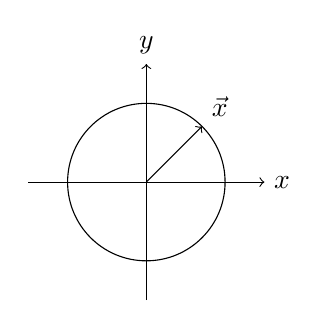
\begin{tikzpicture}
            \draw[->] (-1.5, 0) -- (1.5, 0) node[right] {\( x \)};
            \draw[->] (0, -1.5) -- (0, 1.5) node[above] {\( y \)};
            \draw (0, 0) circle (1);
            \draw[->] (0, 0) -- (0.707, 0.707) node[above right] {\( \vec{x} \)};
        \end{tikzpicture}
        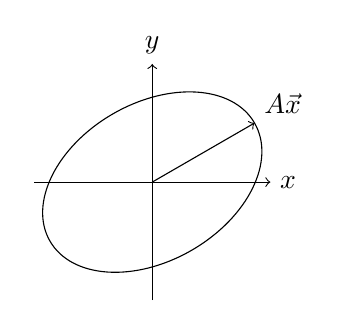
\begin{tikzpicture}
            \draw[->] (-1.5, 0) -- (1.5, 0) node[right] {\( x \)};
            \draw[->] (0, -1.5) -- (0, 1.5) node[above] {\( y \)};
            % Ellipse, rotated 30 degrees
            \draw[rotate=30] (0, 0) ellipse (1.5 and 1);
            \draw[->] (0, 0) -- (1.299, 0.75) node[above right] {\( A\vec{x} \)};
        \end{tikzpicture}
    \end{figure}

    Induced norms are

    \begin{itemize}
        \item The 1-norm \begin{align*}
                  \| A \|_1
                   & = \max_{\| \vec{x} \|_1 = 1} \| A \vec{x} \|_1                    \\
                   & = \max \text{absolute column sum}                                 \\
                   & = \max_{i \leq j \leq n} \left( \sum_{i=1}^n | a_{i, j} | \right) \\
              \end{align*}

        \item The 2-norm
              \begin{align*}
                  \| A \|_2 = \sqrt{{\lambda_{\max} (A^\top A)}}
              \end{align*}

        \item The infinity norm
              \begin{align*}
                  \| A \|_\infty
                   & = \max_{\| \vec{x} \|_\infty = 1} \| A \vec{x} \|_\infty          \\
                   & = \max \text{absolute row sum}                                    \\
                   & = \max_{1 \leq i \leq n} \left( \sum_{j=1}^n | a_{i, j} | \right)
              \end{align*}
    \end{itemize}

    Another useful norm is the \term{Frobenius norm}\index{Frobenius Norm} \[
        \| A \|_F = \sqrt{\sum_{i=1}^n \sum_{j=1}^n {a_{i, j}}^2}
    \]
\end{remark}

\begin{example}
    We revisit the example, where \[
        A = \begin{pmatrix}
            0.780 & 0.563 \\ 0.913 & 0.659
        \end{pmatrix}
    \]

    We have \[
        \| A \|_\infty = 1.572
    \]

    We have defined \[
        \kappa(A) = \| A \| \| A^{-1} \|
    \] but we did not define which norm to use. We could have different condition numbers for different norms. \[
        \kappa_\infty(A) = \| A \|_\infty \| A^{-1} \|_\infty
    \]

    From linear algebra, we know that \textbf{for a \( 2 \times 2 \) matrix} \[
        M = \begin{pmatrix}
            a & b \\ c & d
        \end{pmatrix}
    \] we have its inverse \[
        M^{-1} = \frac{1}{ad - bc} \begin{pmatrix}
            d & -b \\ -c & a
        \end{pmatrix}
    \]

    Thus, we have \[
        A^{-1} = \frac{1}{0.780 \cdot 0.659 - 0.563 \cdot 0.913} \begin{pmatrix}
            0.659 & -0.563 \\ -0.913 & 0.780
        \end{pmatrix}
    \] so \[
        \| A^{-1} \|_\infty \approx 1.693 \times 10^6
    \] and hence the conditional number \[
        \kappa_\infty(A) \approx 2.66 \times 10^6
    \]

    This shows that solving the system is ill-conditioned.

    The relative error in our compute solution is bounded above by \[
        2.66 \times 10^6 \cdot \text{ relative residual in computed solution}
    \]
\end{example}

How small can the condition number be? There is a relation between condition number and near-singularity.

\begin{align*}
    \kappa(A)
     & = \| A \| \cdot \| A^{-1} \| \\
     & \geq \| A A^{-1} \|          \\
     & = \| I \|                    \\
     & = 1
\end{align*}

The condition number is bounded below by 1, and the closer it is to 1, the better conditioned the matrix is.

\begin{example}
    We consider another system \[
        A \vec{x} = \vec{b}
    \] where \[
        \begin{pmatrix}
            1.0 \times 10^{-4} & 1 \\ 1 & 1
        \end{pmatrix}
        \begin{pmatrix}
            x_1 \\ x_2
        \end{pmatrix}
        =
        \begin{pmatrix}
            1 \\ 2
        \end{pmatrix}
    \]

    The exact LU factorization yields \[
        L = \begin{pmatrix}
            1 & 0 \\ 1.0 \times 10^{-4} & 1
        \end{pmatrix}
        \qquad \text{and} \qquad
        U = \begin{pmatrix}
            1.0 \times 10^{-4} & 1 \\ 0 & -9.999
        \end{pmatrix}
    \]

    With forward solve,
    \begin{align*}
        L\vec{y} & = \vec{b} \\
        y_1      & = 1       \\
        y_2      & = -9.998
    \end{align*}
    and then with backward solve,
    \begin{align*}
        U\vec{x} & = \vec{y}           \\
        x_2      & = \frac{9998}{9999} \\
        x_1      & = \frac{1000}{9999}
    \end{align*}

    Now, suppose we get \[
        \bar{L} = \begin{pmatrix}
            1.00 \times 10^0 & 0 \\ 1.00 \times 10^4 & 1.00 \times 10^0
        \end{pmatrix}
        \qquad \text{and} \qquad
        \bar{U} = \begin{pmatrix}
            1.00 \times 10^{-4} & 1.00 \times 10^0 \\ 0 & 1.00 \times 10^4
        \end{pmatrix}
    \]
    and we compute
    \begin{align*}
        \bar{y}_1
         & = 1.00 \times 10^1                                               \\
        \bar{y}_2
         & = fl\left( \frac{2 - 1.00 \times 10^4}{1.00 \times 10^0} \right)
        = -1.00 \times 10^4
         & \text{error}
    \end{align*} and then
    \begin{align*}
        \bar{x}_2 & = 1.00 \times 10^0 \\
        \bar{x}_1 & = 0.00 \times 10^0
    \end{align*}

    While \( \bar{x}_2 \) is accurate, \( \bar{x}_1 \) is not.

    We first check if the matrix is ill-conditioned. We have \[
        \| A \|_\infty = 2
    \] and \[
        \| A^{-1} \|_\infty = \left| \frac{1}{1.0 \times10^{-4} - 1} \right| 2 = 2
    \] so \[
        \kappa_\infty(A) = 4
    \]

    The large error is not due to ill-conditioning.

    We observe that \[
        x_1 = \frac{1.00 - 1.00}{1.0 \times 10^-4}
    \] and we see that we have catastrophic cancellation here.

    We also observe that \[
        A = LU
    \] where \[
        \kappa(L) \approx 1.0 \times 10^8
        \qquad{\text{and}}\qquad
        \kappa(U) \approx 1.0 \times 10^8
    \] so in fact we replaced a well conditioned problem with an ill-conditioned one.
\end{example}

\begin{note}[Fact]
    Whenever multipliers are large (because diagonal elements are relatively small) a loss of accuracy can be observed.
\end{note}

\subsection{Partial Pivoting}

A solution to this issue is to try reordering the equations.

\begin{example}[Cont.]
    We perform row exchange \( R_1 \leftrightarrow \R_2 \), \[
        \begin{pmatrix}
            1 & 1 \\ 1 \times 10^{-4} & 0
        \end{pmatrix} \begin{pmatrix}
            x_1 \\ x_2
        \end{pmatrix} = \begin{pmatrix}
            2 \\ 1
        \end{pmatrix}
    \] and we obtain \[
        L = \begin{pmatrix}
            1.00 & 0 \\ 1.00 \times 10^{-4} & 1.00
        \end{pmatrix}
        \qquad \text{and} \qquad
        U = \begin{pmatrix}
            1,00 & 1.00 \\ 0 & fl(1 - 1 \times 10^{-4}) = 1.00
        \end{pmatrix}
    \] so \[
        \kappa(L) = 1
        \qquad \text{and} \qquad
        \kappa(U) = 4
    \]

    This way, we have a well-conditioned problem.

    We now have \[
        \begin{pmatrix}
            y_1 \\ y_2
        \end{pmatrix} = \begin{pmatrix}
            2.00 \\ 1.00
        \end{pmatrix}
        \qquad \text{and then} \qquad
        \begin{pmatrix}
            x_1 \\ x_2
        \end{pmatrix} = \begin{pmatrix}
            1.00 \\ 1.00
        \end{pmatrix}
    \] which is the correct floating point representation of the exact solution.
\end{example}

\begin{definition}[Pivot Position]\index{Pivot Position}
    The \term{pivot position} is the position in the matrix that is used to eliminate the other elements in the column.
\end{definition}

Suppose we have a matrix \[
    \begin{pmatrix}
        \times & \times & \times & \times & \times \\
        0      & \times & \times & \times & \times \\
        0      & 0      & \times & \times & \times \\
        0      & 0      & \times & \times & \times \\
        0      & 0      & \times & \times & \times \\
    \end{pmatrix}
\]

We interchange \( R_i, R_{r_i} \) using \( P_{i, r_i} \) to move small value off of diagonal.

Choose interchange rows \( r_i \) such that \( \| a_{r_i, i} \| \geq \| a -{j, i} \| \) for all \( j \) from \( i \) to \( n \).

\begin{itemize}
    \item Guarantees multipliers are \( \geq 1 \) in size
    \item Do rows interchanges to ensure multipliers are \( \leq 1 \)
\end{itemize}

\begin{note}[Fact]
    In practice, when row interchanges are used, the Gaussian Elimination algorithm is \textbf{stable}. and guarantees approximate solutions with relative errors \( \frac{\| \vec{r} \|}{\| \vec{b} \|} \approx C_n \cdot \varepsilon_{\text{mach}} \) where \( C_n \) is a small constant dependent on \( n \).

    Thus, \[
        \frac{\| \vec{x} - \vec{x}^* \|}{ \| \vec{x}^* \|} \leq \kappa(A) \cdot \varepsilon_{\text{mach}} \approx \kappa(A) \cdot C_n \cdot \varepsilon_{\text{mach}}
    \]
\end{note}

\begin{remark}[Rule of Thumb]
    Then number of bits of accuracy in the computed solution is approximately \( P - \lceil \log_{\beta} \kappa(A) \rceil \), where \( P \) is the precision of the floating point system.
\end{remark}

\begin{remark}[Terms]
    Row interchanges, row pivoting, and partial pivoting are all the same thing.
\end{remark}

\subsection{Complete Pivoting}

In row pivoting, we only search the columns, while in complete pivoting, we search the entire un-eliminated submatrix \[
    \begin{pmatrix}
        \times & \times            & \times
               & \times            & \times            \\
        0      & \times            & \times
               & \times            & \times            \\
        0      & 0                 & \color{red}\times
               & \color{red}\times & \color{red}\times \\
        0      & 0                 & \color{red}\times
               & \color{red}\times & \color{red}\times \\
        0      & 0                 & \color{red}\times
               & \color{red}\times & \color{red}\times \\
    \end{pmatrix}
\]

Suppose \( | a_{s, t} | > | a_{i, j} | \) for al \( i, j, s, t \) in the un-eliminated submatrix.

In complete pivoting, we interchange to put \( a_{s, t} \) in the pivot position.

Our factorization becomes \[
    PAQ = LU
\] where
\begin{itemize}
    \item \( P \) is a permutation matrix for row interchanges
    \item \( Q \) is a permutation matrix for column interchanges
\end{itemize}
\begin{align*}
    A \vec{x}         & = \vec{b}  \\
    PA QQ^\top \vec{x} = P\vec{b}  \\
    LU Q^\top \vec{x} & = P\vec{b} \\
\end{align*}

\begin{remark}[Considerations]
    Complete pivoting is not always necessary, is more computationally expensive than partial pivoting since we need to search in 2D space instead of 1D space.
\end{remark}